\documentclass[../Main/Main.tex]{subfiles}

\begin{document}
% Qué? (Objetivo)
En luz de las nuevas y populares tendencias en el mundo de la estadística computacional, llamada en ocasiones aprendizaje estadístico u aprendizaje de máquina;\footnote{\textit{machine learning (ML)}} este trabajo plantea como objetivo: estudiar, explicar e implementar un modelo de clasificación supervisada con base en la extensión del modelo \textit{probit} al que se le añade un componente no lineal de bases aditivas. Asimismo, se desarrolla un algoritmo asociado de aprendizaje para la inferencia del modelo y generación de predicción con base en el paradigma bayesiano.\footnote{Es común, hacer una distinción entre el aprendizaje estadístico y el aprendizaje de máquina pues, mientras que los modelos son los mismos, difieren en perspectiva. El aprendizaje estadístico presta mayor atención al aspecto inferencial e interpretación, cuando el aprendizaje de máquina coloca mayor énfasis en la implementación computacional y los resultados.}

% Por qué? 
El modelo hace hace inferencia sobre base en un conjunto de datos y \textit{aprende} sobre los patrones subyacentes que los datos puedan contener para posteriormente, predecir el resultado de variables de respuesta. Este tipo de modelos, han resultado ser de enorme efectividad en ámbitos tan diversos, como lo son la medicina y las finanzas. Bajo esta óptica, se busca que el modelo sea práctico e útil, sin perder de vista el componente teórico que lo sustenta. Por lo tanto, se busca explicar con detalle cada componente del modelo y del algoritmo para que este no sea tratado como una caja negra computarizada.

Los modelos probit son un tipo de regresiones generalizadas, que buscan explicar la clasificación de variables de respuesta $y_i$ binarias (éxito o fracaso, positivo o negativo, etc) con base en un conjunto de covariables $\xni$ que contienen información para cada una de las observaciones $i = 1,\ldots,n$.\footnote{Es usual en la literatura, hablar de \textit{clasificadores} cuando las respuestas son categorías (codificadas en variables discretas) y \textit{regresiones} cuando las variables de respuestas son continuas.} Sin embargo, la relación entre $y_i$ con $\xni$ puede depender de estructuras complejas que no son necesariamente lineales; esto lleva a que la predicción de las respuestas con bsae en las covariables sea difícil. Para sobrepasar esto, al modelo se le agrega un componente no lineal en covariables que permite discernir estos patrones. Como se verá en el trabajo, el modelo induce fronteras no lineales de clasificación en el espacio donde $\xni$ tome valores. En la figura \ref{fig:DiagramaIntro}, se tiene un ejemplo gráfico de tipo de clasificación que lleva a cabo el modelo. Se tienen observaciones del grupo azul y del grupo rojo con una clara separación no lineal en las covariables $x_1$ y $x_2$. El proceso de aprendizaje busca \textit{entrenar}, bajo el paradigma bayesiano, a una función $\eta$ que logre separar este espacio de la mejor forma posible. Esta separación, induce una clasificación binaria (0 y 1 correspondiendo a rojo y azul respectivamente) a través de la función de distribución normal $\Phi$. Con un modelo cuya frontera fuera lineal en covariables, llevar a cabo esta clasificación sería imposible. 

\begin{figure}[h]
  \centering
      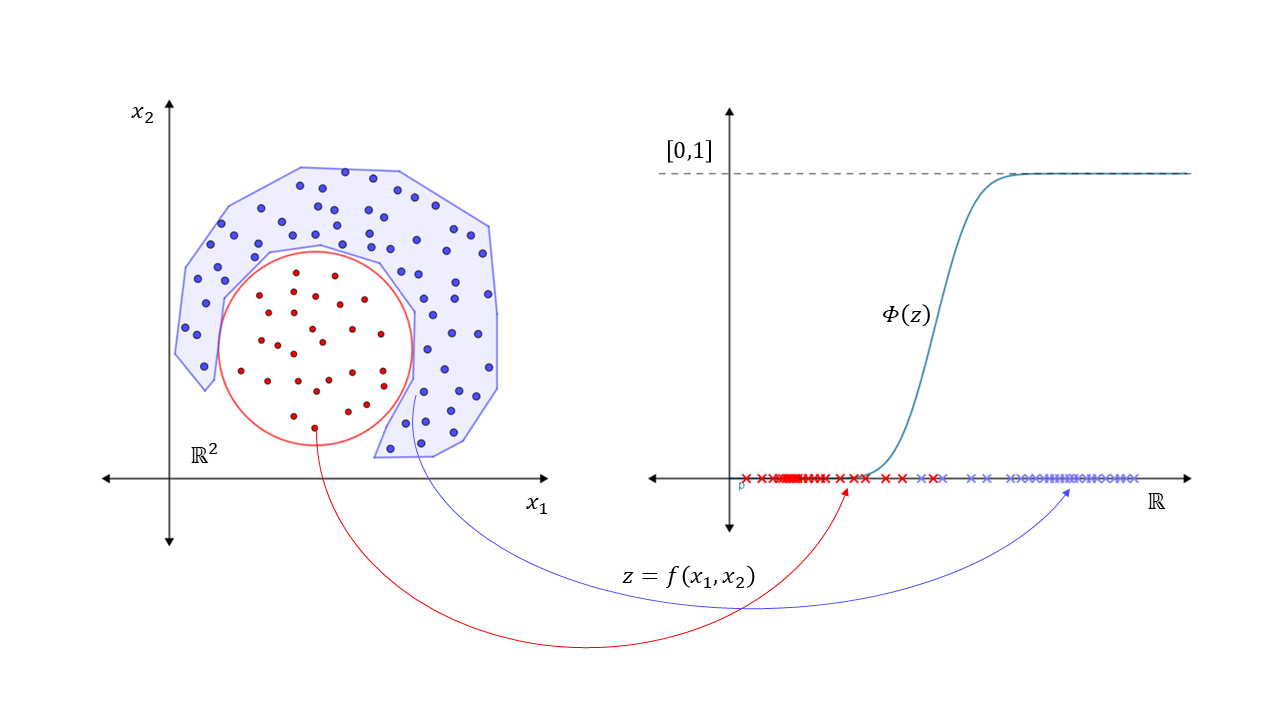
\includegraphics[width = 1\textwidth]{Diagrama_Separabilidad}
  \caption{Diagrama explicativo de un modelo de clasificación probit no lineal}
  \label{fig:DiagramaIntro}
\end{figure}

% De donde y cómo? se plantea la estructura del modelo el capítulo 2
Para llevar a cabo la especificación del modelo, se comienza con una discusión teórica en el capítulo \ref{cap:Modelo}. Primeramente se estudian los modelos lineales generalizados (GLM), específicamente los modelos probit. Los GLM como su nombre lo indica, generalizan las regresiones tradicionales donde la respuesta $y_i$ es escalar ($y_i \in \mathbb{R}$) a regresiones donde la respuesta puede ser discreta o restringida a cierto dominio \autocite{maccullagh1989generalized}. No obstante, los GLM siguen siendo lineales en las covariables pero se pueden flexibilizar usando diferentes ideas. Entre ellas, los modelos aditivos generalizado (GAM) presentadas en \citet{hastie1986generalized}. En estos modelos, la flexibilización se logra transformando a las covariables $\xni$, mediante la función de predicción $\eta$, usando métodos no paramétricos con base en suavizadores. Para este trabajo, se toman esas ideas y se combinan con las de \citet{mallik1998automatic} en las que se opta por darle una forma funcional concreta a $\eta$, correspondiente a una expansión de bases funcionales, particularmente, en polinomios por partes de continuidad y grado arbitrarios.  A lo largo del capítulo, se verá que con principios presentados, se abren las posibilidades en cuanto a modelos y datos sobre los que se pueden hacer regresiones o clasificaciones. %La expansión resultante, tiene la peculiaridad que conectan muchas disciplinas y ramas de las matemáticas que han sido de mucha utilidad no sólo en el campo de la estadística.

% Cómo se implement? Cap. 3
Desarrollado una vez el modelo, el capítulo \ref{cap:BayesAlgoritmo} se concentra en su implementación computacional bajo el paradigma bayesiano de aprendizaje. Por lo tanto, se hace una breve introducción a la escuela bayesiana de la estadística, en particular al apredizaje bayesiano en un contexto de regresión. Este paradigma, responde a que, bajo las ideas de \citet{albert1993bayesian}, el modelo se puede plantear de tal forma que se induce un algoritmo con base en el sampleo de Gibbs. La implementación final, se realiza en el paquete computacional para el lenguaje abierto de programación estadística \verb|R|.\footnote{El desarrollo y explicación del paquete de cómputo se detalla en el Apéndice \ref{ap:Paquete}. El paquete se puede descargar libremente de: \url{https://github.com/PaoloLuciano/bpwpm}}

% Cómo se probo? Cap. 4
En el capítulo \ref{cap:EjYRes}, el modelo se prueba y se valida contra una serie de bases de datos. Primeramente, se hace una breve discusión sobre como evaluar la efectividad y precisión de un modelo como el presentado en este trabajo. Posteriormente, se ejecuta el algoritmo de aprendizaje contra cinco bases de datos simulados con dos covariables ($\xsn_i \in \mathbb{R}^2$). Estas pruebas preliminares, sirven para demostrar las capacidades predictivas del modelo y sobre todo, para hacer más concretas las matemáticas subyacentes, además de poder visualizar las diferentes fronteras flexibles obtenidas por el modelo. Asimismo, en este capítulo se discute la convergencia de las cadenas obtenidas por el muestreador de Gibbs. Para cerrar el capítulo, se replica un escenario real de análisis y modelado usando una base de datos médicos reales de cáncer.

% Y luego? Conclusión Cap. 5
Finalmente, se cierra la discusión en el capítulo \ref{cap:Conclusiones} donde se revisan consideraciones finales y limitantes del modelo, sin embargo, se abre una discusión a posibles extensiones para mejorarlo. Posteriormente, se da un rápido vistazo a modelos relativamente más modernos los cuales han sido capaces de proezas computacionales que se creían imposibles hace algunas décadas. No obstante, se verá que muchos de estos modelos más complejos, son generalizaciones de modelos clásicos y extensiones análogas al trabajo presentado. 
\end{document}